\begin{figure}
    \centering
    \begin{subfigure}{0.32\textwidth}
        \centering
        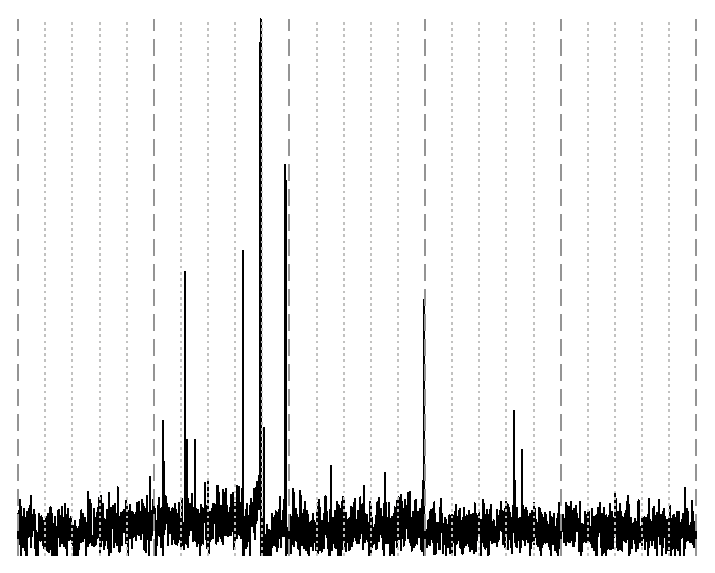
\includegraphics[width=0.95\textwidth,keepaspectratio]{images/b0_peaks/no_B0.eps}
        \caption{Spectral peaks without $B_0$ inhomogeneities ($\mu = 0$Hz)}
        \label{subfig:without B0}        
    \end{subfigure}
    \begin{subfigure}{0.32\textwidth}
        \centering
        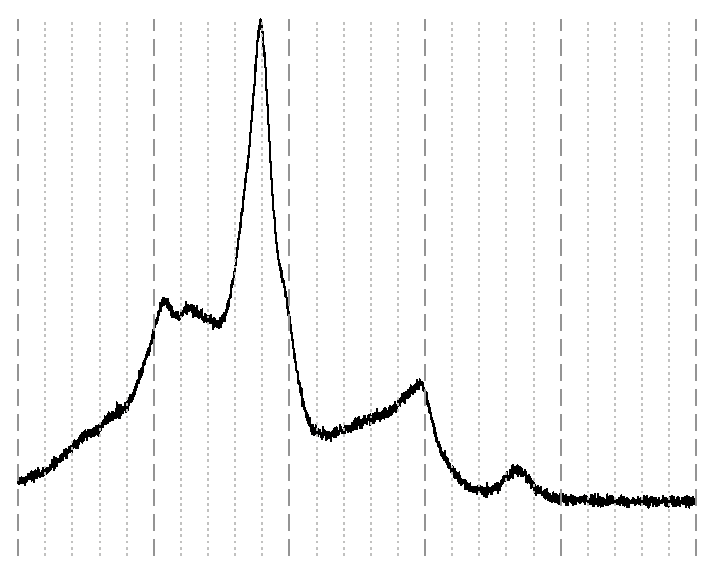
\includegraphics[width=0.95\textwidth,keepaspectratio]{images/b0_peaks/some_B0.eps}
        \caption{Spectral peaks with moderate $B_0$ inhomogeneities ($\mu = 75$Hz)}
        \label{subfig:some B0}        
    \end{subfigure}
    \begin{subfigure}{0.32\textwidth}
        \centering
        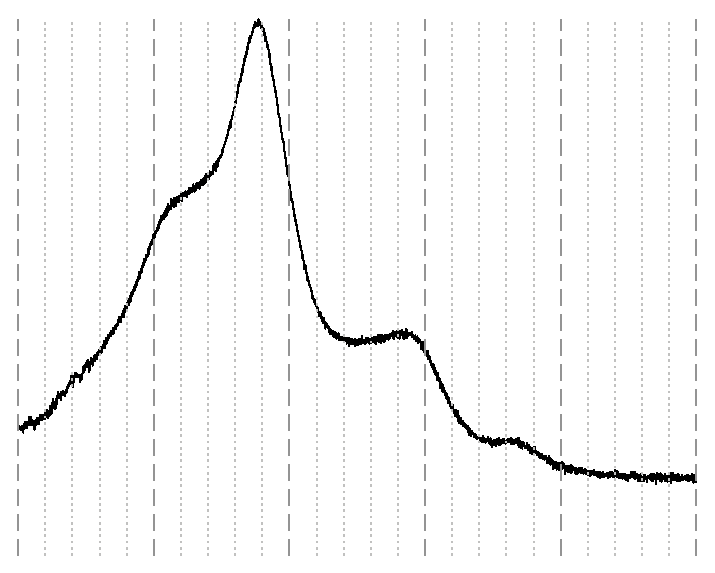
\includegraphics[width=0.95\textwidth,keepaspectratio]{images/b0_peaks/with_B0.eps}
        \caption{Spectral peaks with severe $B_0$ inhomogeneities ($\mu = 175$Hz)}
        \label{subfig:with B0}        
    \end{subfigure}
    \caption{These samples show the effects that can be modeled using the 3D $B_0$ field simulator. In \ref{subfig:without B0}, the spectral peaks have a purely Lorentzian lineshape. In \ref{subfig:some B0}, the lineshape is now Voigtian because the Gaussian term has been added back by the 3D $B_0$ field simulator. In \ref{subfig:with B0}, severe heterogeneities are modeled which produce extremely broad line widths. All three plots use the same x- and y-axes. The observed offsets are caused by the line broadening.}
    \label{fig:B0 effects}
\end{figure}
